\chapter{Encryption}\label{chap:encryption}
In this chapter, we introduce notations for fundamental moves of the most common Rubik's Cube $C_3$. We then work on constructing a group using states of $C_3$. We explain how the encryption protocol is built using the Rubik's Cube and move on to analyze the possible attacks against this encryption protocol. Finally, we layout some improvements to the encryption protocol.

\section{The classic Rubik's Cube}
\par Recall Figure~\ref{fig:solved-cube}, $C_3$ has 3 layers where each layer is formed by 9 smaller cubes, so there are $3 \cdot 9 = 27$ cubes in total. Among those 27 small cubes, 26 small cubes are visible since the center cube is surrounded by them and thus, hidden. If you take apart one Rubik's Cube, you will find that the center cube does not actually exist. In place of the center cube, there is a special structure that holds all other pieces together.
\par We can split the 26 small cubes into three different types. As shown in Figure~\ref{fig:cube-type}, the small cubes in the corners are called ``corner cubes'', which have three visible colored pieces and there are 8 of them in total. The small cubes lie in the middle of each edge are called ``edge cubes'', which have two visible colored pieces and there are 12 of them. Finally, the cubes with a single visible colored piece located at center of each side of the cube are called ``center cubes''. Same as the number of sides a cube has, there are 6 of them.
% ------------------------------ Draw Examples --------------------------------
\begin{figure}[ht]
    \centering
    \begin{minipage}[b]{0.45\textwidth}
        \centering
        \RubikFaceUpAll{Y}
        \RubikFaceFrontAll{G}
        \RubikFaceRightAll{O}
        \ShowCube{5cm}{0.6}{
            \DrawRubikCubeRU
            \draw[line width=2pt, color=blue, <-] (2.5, 1.5) -- (6, 1.5);
            \node at (6, 2) [blue]{\textbf{\textsf{Edge Cube}}};

            \draw[line width=2pt, color=blue, <-] (2, 3.5) -- (2, 4.5);
            \node at (2, 5) [blue]{\textbf{\textsf{Center Cube}}};

            \draw[line width=2pt, color=blue, <-] (3.5, 3.8) -- (5, 5.5);
            \node at (5, 6) [blue]{\textbf{\textsf{Corner Cube}}};
        }
        \setlength{\abovecaptionskip}{0.7cm}
        \caption{Small cube types}\label{fig:cube-type}
    \end{minipage}
    \begin{minipage}[b]{0.45\textwidth}
        \centering
        \RubikFaceUpAll{Y}
        \RubikFaceFrontAll{G}
        \RubikFaceRightAll{O}
        \ShowCube{5cm}{0.6}{
            \DrawRubikCubeRU
            % Right Face
            \draw[line width=2pt, color=blue, <-] (3.5,2) -- (5.5, 2);
            \node at (5, 2.5) [blue]{\textbf{\textsf{Right}}};
            % Left Face
            \draw[line width=2pt, color=blue, <-] (-0.2,2) -- (-1.3, 2);
            \node at (-0.9, 2.5) [blue]{\textbf{\textsf{Left}}};
            % Up Face
            \draw[line width=2pt, color=blue, <-] (2, 3.5) -- (2, 5.5);
            \node at (1.4, 4.8) [blue]{\textbf{\textsf{Up}}};
            % Down Face
            \draw[line width=2pt, color=blue, <-] (2, -0.2) -- (2, -1.5);
            \node at (3, -1.1) [blue]{\textbf{\textsf{Down}}};
            % Front Face
            \draw[line width=2pt, color=blue, <-] (1.5, 1.5) -- (0, -1);
            \node at (-0.5, -1.3) [blue]{\textbf{\textsf{Front}}};
            % Back Face
            \draw[line width=2pt, color=blue, <-] (3.2, 4.2) -- (4, 5.5);
            \node at (4.6, 4.8) [blue]{\textbf{\textsf{Back}}};
        }
        \caption{Rubik's Cube Notation}\label{fig:cube-notation}
    \end{minipage}
\end{figure}
% -----------------------------------------------------------------------------
\par In future discussions, we will refer sides of the Rubik's Cube as faces. To distinguish the six faces, we will call them right face, left face, up face, down face, front face and back face as shown in Figure~\ref{fig:cube-notation}. Following this naming system, we can assign notations to the moves of $C_3$. The most basic move one can do it to rotate a single face of the cube. We use $U$ to denote a clockwise rotation of the up face. That is looking at the up face, turn it $90^\circ$ clockwise. Similarly, we use letters $R$, $L$, $D$, $F$ and $B$ to denote the clockwise $90^\circ$ rotation of the corresponding faces. For each of these six moves, there are three possible angles of rotation, which are $90^\circ$ clockwise, $180^\circ$ clockwise and $270^\circ$ clockwise. In total there are $6 \cdot 3 = 18$ possible moves and we will call these the \textit{fundamental moves}.
\begin{figure}[ht]
    \centering
    \begin{minipage}{0.9\textwidth}
        \centering
        \RubikCubeSolvedWY
        \ShowCube{2cm}{0.5}{\DrawRubikCubeRU}
        \quad\Rubik{U}\quad
        \RubikRotation{U}
        \ShowCube{2cm}{0.5}{\DrawRubikCubeRU}
        \quad\Rubik{Up}\quad
        \RubikRotation{Up}
        \ShowCube{2cm}{0.5}{\DrawRubikCubeRU}
        % Add a little space between the two graphs.
        \vspace*{10px}
    \end{minipage}
    \begin{minipage}{0.9\textwidth}
        \centering
        \RubikCubeSolvedWY
        \ShowCube{2cm}{0.5}{\DrawRubikCubeRU}
        \RubikRotation{U, U}
        \quad
        \SequenceBraceA{U2}{\ShowSequence{}{\Rubik}{\SequenceLong}}
        \quad
        \ShowCube{2cm}{0.5}{\DrawRubikCubeRU}
    \end{minipage}
    \caption{Rotation example}\label{fig:cube-rotation-example}
\end{figure}
\par To represent the clockwise $180^\circ$ rotation of the corresponding faces, we simply add a number 2 after the capital letters. Therefore, $U2$ represents the move where we face the up face and rotate it $180^\circ$ clockwise. For the $270^\circ$ clockwise rotation, which is same as a $90^\circ$ counterclockwise rotation, we add an apostrophe after the capital letter to denote it. Then $U'$ represents the move where we face the up face and rotate it $90^\circ$ counterclockwise. All above notations defined are illustrated in Figure~\ref{fig:cube-rotation-example}.
\begin{figure}[ht]
    \centering
    \begin{minipage}{0.48\textwidth}
        \centering
        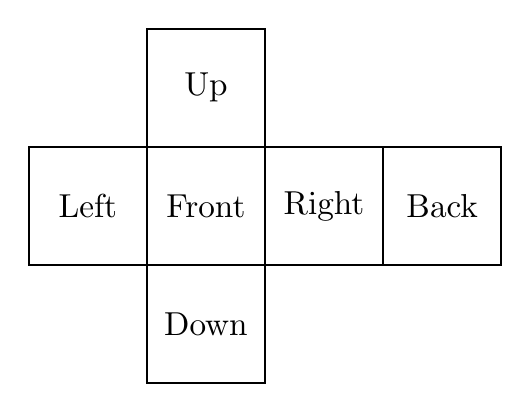
\begin{tikzpicture}[scale=0.5]
            \draw[thick] (4.5,-0.5) -- (7.5,-0.5) -- (7.5,-9.5) -- (4.5,-9.5) -- cycle;
            \draw[thick] (1.5,-3.5) -- (13.5,-3.5) -- (13.5,-6.5) -- (1.5,-6.5) -- cycle;
            \draw[thick] (10.5,-3.5) -- (10.5,-6.5);
            \node[thick, scale=1.2] at (6,-2) {Up};
            \node[thick, scale=1.2] at (3,-5) {Left};
            \node[thick, scale=1.2] at (6,-5) {Front};
            \node[thick, scale=1.2] at (9,-5) {Right};
            \node[thick, scale=1.2] at (12,-5) {Back};
            \node[thick, scale=1.2] at (6,-8) {Down};
        \end{tikzpicture}
    \end{minipage}
    \begin{minipage}{0.48\textwidth}
        \centering
        \RubikCubeSolvedWY
        \RubikRotation{T,F,R,D,B,L,Tp,Fp,Rp,Dp,Bp,Lp}
        \ShowCube{7cm}{0.5}{\DrawRubikCubeF}
        \vspace{0.5cm}
    \end{minipage}
    \begin{minipage}{0.99\textwidth}
        \centering
        \RubikRotation{T,F,R,D,B,L,Tp,Fp,Rp,Dp,Bp,Lp}
        \ShowSequence{}{\Rubik}{\SequenceLong}
    \end{minipage}
    \caption{A state of the Rubik's Cube}\label{fig:cube-state-example}
\end{figure}
\par As we mentioned earlier, we refer each possible shuffling result of the cube as a state. Figure~\ref{fig:cube-state-example} is one possible state of the cube. The shuffling can be any combination of the fundamental moves applied to a solved cube. Each state of the cube is unique, though infinitely many different shufflings could reach it. Suppose we are at a state $S$ that can be reached by series of fundamental moves $M$. Then if we add ``$R\,R\,R\,R$'' at the end of $M$, we are still at state $S$ since ``$R\,R\,R\,R$'' simply rotates the right face $360^\circ$ clockwise and does not actually change it. In fact, we can insert any number of ``$R\,R\,R\,R$'' anywhere in $M$. Also, we do not have to always use $R$, any four fundamental moves will rotate one face of the cube by a multiple of $360^\circ$ and hence do not modify the cube. Thus we have infinitely many ways to reach $S$.
\par We now want to show that we can make the set of states of $C_3$ into a group. Let us denote the group as $G_3$ where the group operation is $*$, and each element of $G_3$ is a state. Though arguments below correspond to $C_3$, we can use them to construct group $G_n$ for states of an arbitrary cube $C_n$ in a similar fashion. 
\par Assume $S_1$ and $S_2$ both represent a state of the classic 3 by 3 by 3 cube, that is $S_1, S_2 \in G_3$. Assume $S_1$ can be reached by a series of moves $M_1$ applied to the solved cube and similarly $S_2$ can be reached by a series of moves $M_2$ applied to the solved cube. Then $S_1 * S_2$ is the state you could reach to by first applying $M_1$ and then $M_2$ to the solved cube, or equivalently, you can directly apply $M_2$ to $S_1$. Then it is obvious that if we pick a different $M'$ which takes us from the solved cube to $S_1$, $S_1 * S_2$ still gives us the same result. Therefore the operation $*$ is well defined. We now can show a simple proof that $G_3$ is indeed a group under $*$. \\
\textit{Claim}: $G_3$ is a group under $*$.
\begin{proof}[Proof:]\item
    \begin{itemize}
        \item Show closure. \\
        Suppose we have $S_1, S_2 \in G_3$. From above description, we see that $S_1 * S_2$ can be reached by combining two series of moves. Thus $S_1 * S_2$ is indeed a state of the cube. Therefore $G_3$ is closed.
        \item Show identity. \\
        The solved cube is the identity and we denote it as $e$. It represents the "empty" move. Suppose we have $S \in G_3$, then $e*S$ means do nothing and move to $S$. Similarly $S*e$ means applying nothing to $S$. Therefore the solved cube is the identity.
        \item Show associativity. \\
        Suppose we have $S_1, S_2, S_3 \in G_3$. Clearly $(S_1 * S_2) * S_3 = S_1 * (S_2 * S_3)$ since the order we apply those moves does not change even if we combine two states together. 
        \item Show inverse. \\
        Suppose we have $S \in G_3$ and $S$ can be reached by a series of moves $M$ applied to the solved cube. Each move in $M$ is one of the 18 possible fundamental moves. All fundamental moves have their inverses. For example, $U$ can be reversed by $U'$ and $U2$ can be reversed by $U2$. Thus there must exist a series of moves $M'$ that reverses $M$. We can find $M'$ by inverting of all movements in $M$ in reverse order. That is, the move that was done the last shall be undone first. Applying $M'$ to the solved cube to obtain $S'$ then $S*S' = S'*S = e$.
    \end{itemize}
    Therefore $(G_3, *)$ is a group.
\end{proof}

\section{The design principle}
\par ``Do not worry about your difficulties in Mathematics. I can assure you mine are still greater.'' This is one of my favorite quote from Albert Einstein. Let us assume that we now want to secretly pass this quote to someone using the Rubik's Cube. The general idea is, as we mentioned in Chapter~\ref{chap:introduction}, instead of letting each cubie to hold a color, we use cubies to hold letters. We then need to agree on an order that we put the letters in. As long as we are consistent, we can order the six faces in any way we desire. Once we fill all the faces, we can shuffle the cube to obtain the ciphertext. But before we get started on filling the cube with letters, some pre-processing to the plaintext is essential. We want to remove blanks and punctuations, since their existences in the ciphertext leaks important information about the plaintext. An eavesdropper can count the number of blanks to deduce how many words were encrypted. Afterwards, we also want to make sure all the letters are either capitalized or lower cased. Here we choose to capitalize everything and the processed string looks like the following:
\begin{center}
    \texttt{DONOTWORRYABOUTYOURDIFFICULTIESINMATHEMATICSI} \\
    \texttt{CANASSUREYOUMINEARESTILLGREATERALBERTEINSTEIN}
\end{center}
Since we are using the classic Rubik's Cube $C_3$, we can put $3 \cdot 3 = 9$ letters on each face. At one time, we can use the cube to encrypt at most $9 \cdot 6 = 54$ letters. Our message is too long to fit, but we can take 54 letters and encrypt them first. Here are the first 54 letters split into chunk of 9:
\begin{center}
    \textcolor{blue}{\texttt{DONOTWORR}} \; \textcolor{red}{\texttt{YABOUTYOU}} \; \textcolor{blue}{\texttt{RDIFFICUL}} \;
    \textcolor{red}{\texttt{TIESINMAT}} \; \textcolor{blue}{\texttt{HEMATICSI}} \; \textcolor{red}{\texttt{CANASSURE}}
\end{center}
\par Let us agree on the order of filling the letters as the following: up face $\rightarrow$ front face $\rightarrow$ right face $\rightarrow$ down face $\rightarrow$ back face $\rightarrow$ left face. The cube with letters filled is displayed in Figure~\ref{fig:cube-plain-text}.
\begin{figure}[ht]
    \centering
    \begin{minipage}{0.45\textwidth}
        \centering
        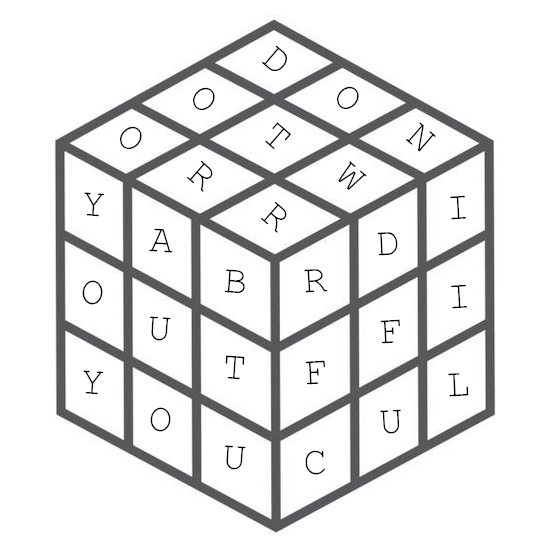
\includegraphics[width=6cm]{figures/encryption/cube_plain_text.png}
        \caption{Cube with plaintext}\label{fig:cube-plain-text}
    \end{minipage}
    \begin{minipage}{0.45\textwidth}
        \centering
        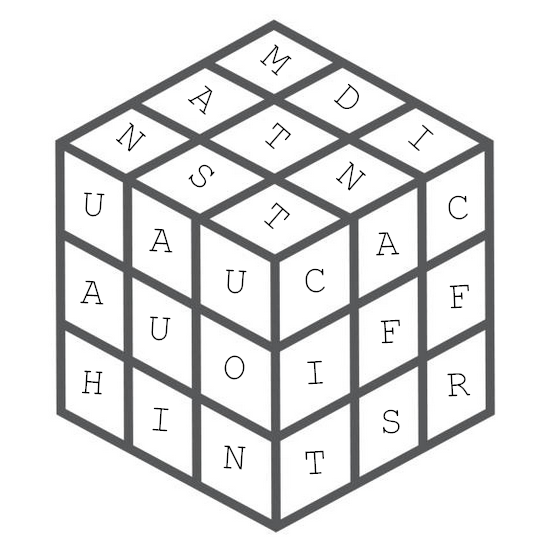
\includegraphics[width=6cm]{figures/encryption/cube_cipher_text.png}
        \caption{Cube with ciphertext}\label{fig:cube-cipher-text}
    \end{minipage}
\end{figure}
We then need to determine a sequence of fundamental moves as our encryption key, which we denote as $k$. Suppose we apply ``$R\,U\,B2\,L'\,D2\,F\,R'\,D\,B\,L2\,$'' to the cube. The shuffled cube is shown as Figure~\ref{fig:cube-cipher-text}. To obtain the entire ciphertext $c$, which is shown below, we simply read out all the letters the same order we put them in. 
\begin{center}
    \textcolor{blue}{\texttt{MDIATNNST}} \; \textcolor{red}{\texttt{UAUAUOHIN}} \; \textcolor{blue}{\texttt{CACIFFTSR}} \; 
    \textcolor{red}{\texttt{YWLTIEBRM}} \; \textcolor{blue}{\texttt{EOCOTROID}} \; \textcolor{red}{\texttt{ESIOSUYAR}}
\end{center}
\par We now send the ciphertext $c$ to the receiver. It is crucial for us to have shared the key secretly with the receiver. We will discuss a method to do so in Chapter~\ref{chap:exchange}. Upon receiving the ciphertext, the receiver can decrypt the ciphertext by first finding the inverse of the key, which we denote as $k'$. By following the step described in proving the inverses of group $G_3$, we find $k'$ is ``$L2\,B'\,D'\,R\,F'\,D2\,L\,B2\,U'\,R'\,$''. Then the receiver can fill the cube with the ciphertext and apply $k'$ to the cube.
\par Let us take a closer look at what happened during the encryption. We notice that all letters that were in plaintext are present in the ciphertext. However most of them ended up in different locations. If we observe the center of each face, we can find that they all remained in the same places. This is not a coincidence since none of the basic moves changes the center. Therefore among the 54 letters, at most 48 letters can be permuted.

\section{Brute force attacks}
\par Let us consider the brute force attacks against this protocol. There are two relative obvious ways of doing so. From above discussion, we know the ciphertext is just one possible permutation result of 48 letters within the plaintext. Thus if we list out all elements of $S_{48}$, the permutation group on 48 elements, and apply each to the ciphertext, one of the permutations must revert the ciphertext back to the plaintext.
\par Though the group $S_{48}$ has $48! \approx 1.24 \cdot 10^{61}$ elements, later in this thesis, we will show that not all those permutations are needed to be checked. Even though Rubik's Cube permutes 48 elements, the size of the group $G_3$ is smaller than $S_{48}$, since there are invalid states that cannot be reached by series of fundamental moves. Potentially you can take the cube apart and put it back together to get to a invalid state. We will talk about what states are invalid and why they are invalid in Chapter~\ref{chap:structure} when we explore more about the group structure.
\par The other possible attack is to search the inverse of the encryption key. Without knowing the length of the key we used, the attacker can start with trying out all combination of fundamental moves with length of 1, length of 2 and so on. For each combination the attacker selects, he/she applies it to the cube and observe if the result makes sense. As an example, there are $18^2$ possible keys with length of 2 since every time the attacker can pick one from the 18 fundamental moves. It follows that, in our example, the number of keys the attacker needs to go through is upper bounded by $\sum_{i=1}^{10}18^i \approx 3.78 \cdot 10^{12}$.
\par By comparing the two brute force attacks described above, we notice that finding the inverse of the key would be easier for the attacker. It seems that there is a straightforward approach to make this brute force attack infeasible, which is to increase the key length. Instead of using a key with a length of 10 fundamental moves, we can randomly pick a key that is formed by 1000 fundamental moves. Then if we follow above methods, we will find the number of keys the attacker have go through being bounded by $\sum_{i=1}^{1000}18^i \approx 1.98 \cdot 10^{199}$ which is obviously a way larger number. However this approach will not work as expected due the existence of the God Number.

\section{The God Number}
\par We know that mathematicians love the Rubik's Cube as they are amazed by how such a seemingly regularly puzzle can hold so many secrets. Ever since the problem is invented, perhaps the biggest mystery of all is the upper bound for number of fundamental moves to reach to all possible states. The lower bound is proved earlier in 1995 by Michael Reid\cite{god}. Reid found that the superflip, which keeps all small cubes in their solved locations but flips the orientation of all edge cubes, as displayed in Figure~\ref{fig:superflip} requires at least 20 fundamental moves. 
\begin{figure}[ht]
    \centering
    \RubikCubeSolvedWY
    \RubikRotation{\superflip}
    \ShowCube{8cm}{0.7}{\DrawRubikCubeSF}
    \caption{Superflip}
    \label{fig:superflip}
\end{figure}
It took mathematicians about 30 years to prove that this is an upper bond. We formally define the God Number as:
\newpage
\begin{definition}\textbf{The God Number} \\
    Let $m(S_1, S_2)$ denote the minimum number of fundamental moves to transform $C_3$ from $S_1$ to $S_2$. Then the God Number is $max\{m(S_1, S_2) \;|\; S_1, S_2 \in G_3\}$.
\end{definition}
\par With about 35 CPU-years of idle computer time donated by Google, a team of researchers essentially solved every position of the Rubik's Cube and showed in 2010 that the God Number is 20\cite{god}. Another way to express the meaning of the God Number is that any series of fundamental moves with length longer than 20 can be reduced to a series of fundamental moves with length less or equal to 20. Thus, we can not find two states in the Rubik's Cube that are more than 20 fundamental moves away. We can also say that the Rubik's Cube group $G_3$ we defined has a diameter of 20 fundamental moves.
\par Therefore, even if we have chosen a key with length of a thousand fundamental moves, the attacker will find the inverse of the key with only searching for keys that having length of 20 fundamental moves or less. That is, the number of keys the attacker has to go through is really bounded by $\sum_{i=1}^{20}18^i \approx 1.35 \cdot 10^{25}$, regardless to the key length we choose. It follows that the key search attack will almost always be easier than the attack on finding inverse of the permutation. It is also worthwhile to note that the God Number for larger cubes is unknown, so we are not able to perform a similar analysis on larger cubes.

\section{Improvements}
\par In this section, we discuss solutions that prevent the key from collapsing and other tweaks to our design to improve the security of our protocol in general. First, let us observe some additional features provided by Rubik's Cubes that we overlooked. 
\par Suppose we fill a letter E in the right up corner cubie on the front face of the cube as shown in Figure~\ref{fig:cube-letter}.
\begin{figure}[ht]
    \centering
    \begin{minipage}{0.49\textwidth}
        \centering
        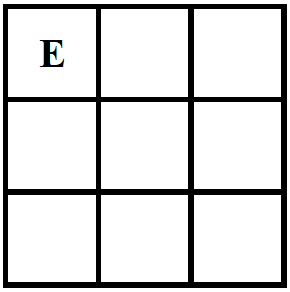
\includegraphics[width=4cm]{figures/encryption/cube_face_letter.png}
        \caption{Front face with letter}\label{fig:cube-letter}
    \end{minipage}
    \begin{minipage}{0.49\textwidth}
        \centering
        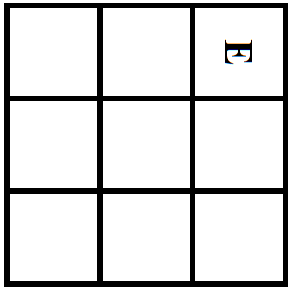
\includegraphics[width=4cm]{figures/encryption/cube_face_letter_rotate.png}
        \caption{Front face with rotated letter}\label{fig:cube-letter-rotate}
    \end{minipage}
\end{figure}
If we rotate the front face 90 degrees clockwise, as shown in Figure~\ref{fig:cube-letter-rotate}, we can find the position of letter \textbf{E} changes. However, we also notice that the orientation of \textbf{E} changes. Since anyone who reads English can still recognize those letters even if their direction changed, we omitted this feature while developing the encryption scheme. To benefit from this feature, we can use something that rotates while the cube faces rotate. Therefore, instead of putting the letters, we can put four bits into each cubie, where each corner of the cubie holds one bit. We need to agree on an order of placing those bits, for example: left up corner $\rightarrow$ right up corner $\rightarrow$ right down corner $\rightarrow$ left down corner, so we get a complete cycle here. Assume that we are putting integers from 1 to 36 on one face of the cube in the order, the face will look like what is displayed in Figure~\ref{fig:bit-order}.
\begin{figure}[ht]
    \centering
    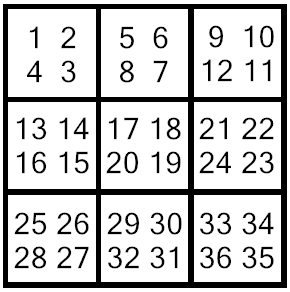
\includegraphics[width=4cm]{figures/encryption/bit_order.png}
    \caption{Bit ordering}\label{fig:bit-order}
\end{figure}
We now can run the above experiment again with input ``1000.'' Following the order we agreed, we put the bits into the left up corner cubie on the front face as shown in Figure~\ref{fig:cube-bit} and the face after the rotation is displayed in Figure~\ref{fig:cube-bit-rotate}.
\begin{figure}[ht]
    \centering
    \begin{minipage}{0.49\textwidth}
        \centering
        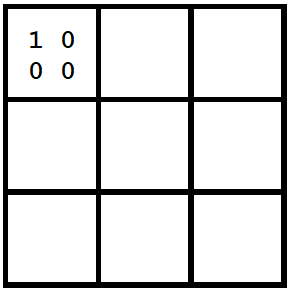
\includegraphics[width=4cm]{figures/encryption/cube_face_bit.png}
        \caption{Front face with bits}\label{fig:cube-bit}
    \end{minipage}
    \begin{minipage}{0.49\textwidth}
        \centering
        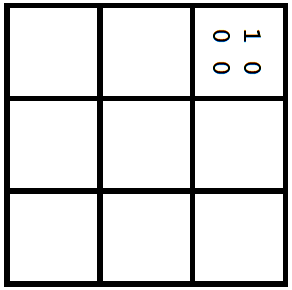
\includegraphics[width=4cm]{figures/encryption/cube_face_bit_rotate.png}
        \caption{Front face with rotated bits}\label{fig:cube-bit-rotate}
    \end{minipage}
\end{figure}
If we read out the bits the same order we put them in, we get ``0100'', which is different from the original input. Hence using bits helps us benefit from the face rotations of the Rubik's Cube. Though this method does not directly address the key collapsing issue, it gives us more flexibility to modify the encryption protocol. We will make further improvements based on this setting.
\par One obvious reason the key would collapse is because some fundamental moves commute with each other. Clearly, each fundamental move commutes with itself regardless of the angle; for example $R$, $R2$ and $R'$ commute with each other. Also, the moves that rotate opposite sides commute with each other. For instance $R$, $R2$ and $R'$ commute with $L$, $L2$ and $L'$. Suppose we find a series of moves within a random key of length 15 as ``$R2\,L2\,R2\,L\,L\,$''. Since those moves commute, they are equivalent to ``$R2\,R2\,L2\,L\,L\,$''. In words, what this chunk of key does is rotating the right face $360^\circ$ clockwise and then rotating the left face $360^\circ$ clockwise, which has precisely no effect on the cube. Thus we can merely remove this chunk from the random key and its length will collapse down from 15 to 10. 
\par To resolve this issue, we can shift the content to the right by one bit each time before we apply a move to the cube. Each one of the bits will move to the next position following the order they were put in. For example, recall Figure~\ref{fig:bit-order}, the bit at location of number $n$ will be shifted to the location of number $n + 1$. Notably, the last bit on one face will become the first bit on the face next to it. For instance, the last bit on the up face will become the first bit on the front face.
\begin{figure}[ht]
    \centering
    $\xrightarrow{\text{fill bits\;\;}}$
    \begin{minipage}{0.3\textwidth}
        \centering
        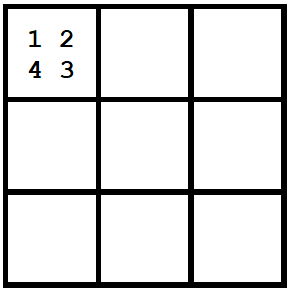
\includegraphics[width=3.5cm]{figures/encryption/bit_start.png}
    \end{minipage}
    $\xrightarrow{\text{shift bit}}$
    \begin{minipage}{0.3\textwidth}
        \centering
        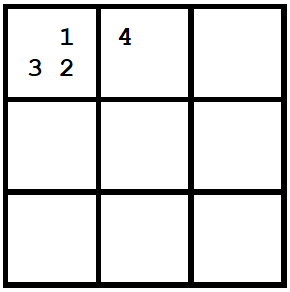
\includegraphics[width=3.5cm]{figures/encryption/bit_shift_one.png}
    \end{minipage}
    \\ $\xrightarrow{\text{apply }F}$
    \begin{minipage}{0.3\textwidth}
        \centering
        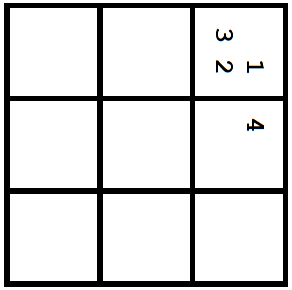
\includegraphics[width=3.5cm]{figures/encryption/bit_rotate_one.png}
    \end{minipage}
    $\xrightarrow{\text{shift bit}}$
    \begin{minipage}{0.3\textwidth}
        \centering
        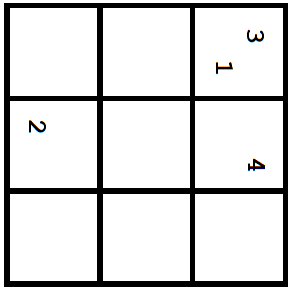
\includegraphics[width=3.5cm]{figures/encryption/bit_shift_two.png}
    \end{minipage}
    \\ $\xrightarrow{\text{apply }F'}$
    \begin{minipage}{0.3\textwidth}
        \centering
        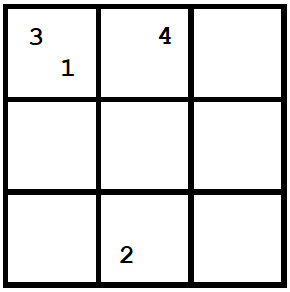
\includegraphics[width=3.5cm]{figures/encryption/bit_rotate_two.png}
    \end{minipage}
    \caption{The bit shift method}\label{fig:bit-shift}
\end{figure}
As shown in Figure~\ref{fig:bit-shift}, we put ``1234'' in the right up corner of the front face and apply moves $F$ and $F'$ to the cube. We follow the procedures defined above and shift the bits before applying each move. Though ``1234'' is not a legal input to the Rubik's Cube encryption, we use it to clearly illustrate where each bits travels to. By observing the front face in the last row of Figure~\ref{fig:bit-shift}, we find the locations of all bits changed, though $F$ and $F'$ cancel each other out. Among the four bits, two bits even moved to other cubies. Therefore, with the shift, the bits travel around even when moves commute and cancel each other out as fundamental moves. We believe this method effectively prevents the key from collapsing. Also, this method addresses the "fixed center" issue since the shift affects bits that are held by center cubies.
\par To examine the modified encryption protocol, we can try to encrypt my favorite quote from Einstein again with the modified Rubik's Cube encryption. Notice we first need to convert the English letters to their ASCII representations, so each letter will be 8 bits long. Since $C_3$ can hold 216 bits, we can encrypt $\frac{216}{8} = 27$ letters at once. The first 27 letters are ``\texttt{DONOTWORRYABOUTYOURDIFFICUL}'' and the following is its binary representation:
\begin{center}
    010001000100111101001110010011110101010001010111010011110101001001010010
    010110010100000101000010010011110101010101010100010110010100111101010101
    010100100100010001001001010001100100011001001001010000110101010101001100
\end{center}
We can use the same key ``$R\,U\,B2\,L'\,D2\,F\,R'\,D\,B\,L2\,$'' to encrypt the plaintext but this time we will account for the shift before applying each move to the cube. The encrypted ciphertext is:
\begin{center}
    001110100110100110111010011100000010100011101111111010011111101111011101
    001000011001100011110000001000111111110110000010010100000000011010001000
    010011101010011010010100110001010100101000000110100110001100011010100001
\end{center}
From Figure~\ref{fig:bit-order}, we see that the center of the cube face goes from the 17th position to the 20th position. We thus can find, in the plaintext, the center of the up face holds $1001$ and this value changed to $0111$ after the encryption. Among the four bits, only one bit actually remained the same. So in this particular example, the shifting bits is effectively helping to change the bits held by the center cubes.
\par We can convert the ciphertext back to ``letters''. But since we can no longer guarantee that each chunk of 8 bits still represent a value that is less than or equal to 127, we need to rely on the extended ASCII table as shown in Figure~\ref{fig:ascii} to convert the ciphertext back to ``letters.'' 
\begin{figure}
    \centering
    
\includegraphics[width=12cm]{figures/encryption/ascii.png}
    \caption{Extended ASCII table}
    \label{fig:ascii}
\end{figure}
The following characters are the results of the conversion: ``:i$\|$p($\cap\uptheta\surd\blacksquare$!\"{y}$\equiv$\#$^2$\'{e}P\;\^{e}N$^a$\"{o}$\dagger$J\;\"{y}$\vdash$\'{\i}.'' As one can notice that while we are using the extended ASCII, many more special characters will be involved. We find that the only common letter that exists in both the ciphertext and the plaintext is the letter N, but the location of it has changed. 
\par The essence of the shift on the bits is just a permutation. We described the shift as a minimum working example, but we are free to pick any permutation on the 216 bits as long as we can specify it. To add more security, we can select a more complex permutation and secretly share it as part of the key with other trusted parties.

\section{Encrypt long messages}
\par When we first defined the Rubik's Cube encryption, we noticed that we could not use it to encrypt the entire quote, since the Rubik's Cube can only fit a certain amount of the plaintext at once. In real life, we may often need to encrypt messages that are much longer. Thus, we introduce two methods that help us encrypt long messages.
\par The first method is designed targeting the Rubik's Cube encryption. We have been using $C_3$ for the encryption, but in Chapter~\ref{chap:introduction} we mentioned that cubes with larger side length do exist. Hence we can use a Rubik's Cube with greater side length to extend the size of the message we are capable of encrypting. Suppose we instead use a 10 by 10 by 10 Rubik's Cube, denoting as $C_{10}$, we can encrypt $10^2 \cdot 6 \cdot 4 = 2400$ bits at once. If we are using ASCII representation of English letters, we can encrypt 300 letters at once. The advantage of using more giant cubes is that we make both brute force attacks we discussed earlier more challenging to succeed. To begin with, when the side length of the Rubik's Cube gets greater, we permute much more bits. For $C_{10}$, we permute 2400 bits, and thus the attacker has to search through group $S_{2400}$ which has $2400!$ elements. For an arbitrarily large cube $C_n$, we permute $24 \cdot n^2$ bits. It follows that if the attacker wants to search through the permutation group, he/she has to go through $(24 \cdot n^2)!$ possibilities. Therefore finding the inverse of the permutation will require much more computations as the side length of the cube increases. Besides, more giant cubes have more than just 18 fundamental moves. For example, $C_{10}$ has 180 fundamental moves. Since each time there are much more fundamental moves to select, finding the inverse of the key will get a lot harder too.
\par There are also two vulnerabilities of this approach. The first one is that we still cannot encrypt an arbitrarily long message. Once we fix a cube length, say 20, we do not want to change it during the communications. The reason is that, while modifying the size of the cube, we are changing the key space as well. That is the fundamental moves we can select for $C_3$ and $C_{20}$ are obviously different. However, for private key encryptions, we commonly exchange the secret key once before building the secure channel between parties, and we use the same key for all of the following communications. Secondly, we may end up wasting a lot of space when we need to encrypt a relatively short message since the cube size is fixed.
\par A more general approach that works for message with arbitrary length $l$ is called the cipher block chaining (CBC) mode, which the is the most commonly used mode of operation. Let us first introduce the operation ``XOR'' is denoted as $\oplus$ and it is also called ``exclusive or''. It gains the name "exclusive or" because it excludes the case when both operands are true.
\begin{table}[ht]
    \centering
    \begin{tabular}{|c|c|c|}
        \hline Input A & Input B & A $\oplus$ B \\ \hline\hline
        1 & 1 & 0 \\ \hline 
        1 & 0 & 1 \\ \hline
        0 & 1 & 1 \\ \hline
        0 & 0 & 0 \\ \hline
    \end{tabular}
    \caption{XOR truth table}\label{tab:xor-truth-table}
\end{table}
``XOR'' is a logical operation that outputs true only when inputs differ. We build the truth table for it as shown in Table~\ref{tab:xor-truth-table}.
\par In CBC mode, each block of plaintext is XORed with the previous ciphertext block before being encrypted as shown in Figure~\ref{fig:cbc-encryption}.
\begin{figure}[ht]
    \centering
    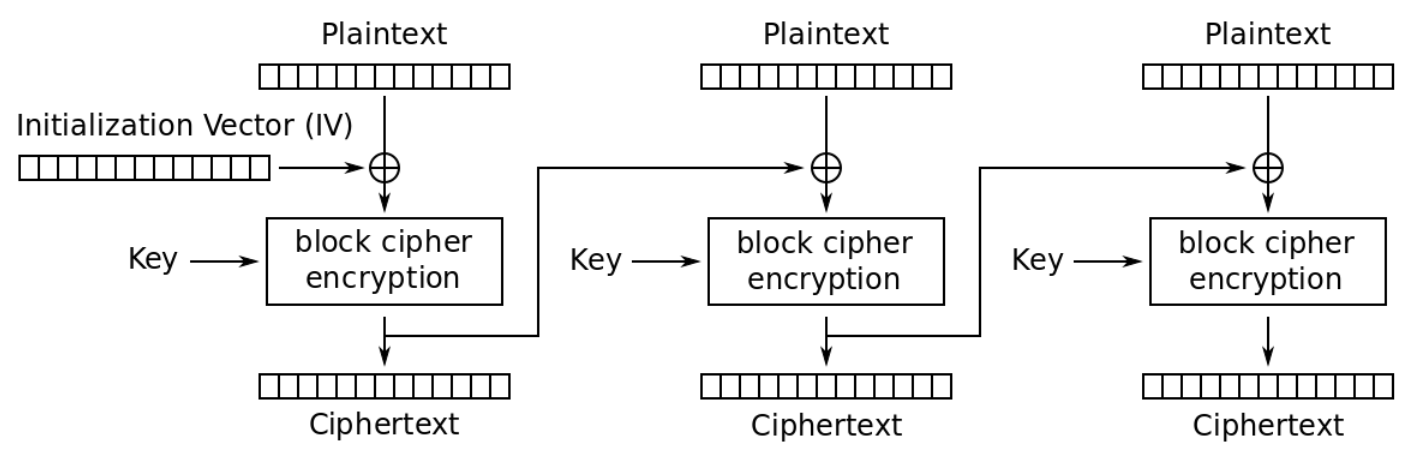
\includegraphics[width=14cm]{figures/encryption/CBC_encryption.png}
    \caption{CBC mode encryption\cite{cbc_enc}}\label{fig:cbc-encryption}
\end{figure}
Hence each ciphertext block depends on all plaintext blocks processed up to that point. To make each message unique, we can use an initialization vector to XOR with the first block. Assume in total there are $k$ blocks of plaintexts $(m_0, m_1, ..., m_k)$ needed to be encrypted, the output will be $k$ blocks of ciphertexts $(c_0, c_1, ..., c_k)$.
\begin{figure}[ht]
    \centering
    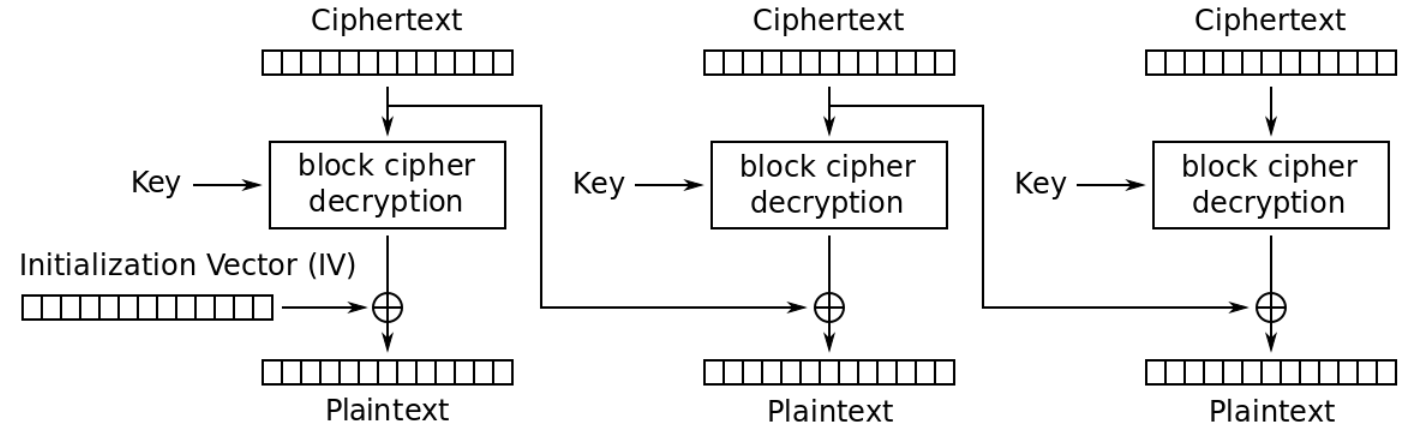
\includegraphics[width=14cm]{figures/encryption/CBC_decryption.png}
    \caption{CBC mode decryption\cite{cbc_dec}}\label{fig:cbc-decryption}
\end{figure}
Giving all the ciphertexts, to retrieve $m_x$ where $2 \leq x \leq k$, we decrypt $c_x$ with the key and then XOR the result with $c_{x-1}$ to get $m_x$ back as shown in Figure~\ref{fig:cbc-decryption}. The first ciphertext $c_1$ is unique since we need to XOR its decryption result with the initialization vector to recover $m_1$. Though this general approach is easy to manage, it has some potential vulnerabilities such as one bit wrong in the $x_{th}$ ciphertext will generate errors in all blocks after it.
\par Finally, for both approaches discussed above, we have to deal with one more issue. In most times, we probably will not have a message that fits perfectly with the encryption scheme we have. Suppose we have a message $m$ with length of 2000 bits and we are using $C_{10}$ to encrypt it. Recall that $C_{10}$ offers 2400 spaces for bits and thus we have 400 spare spaces. We want to agree on a simple padding algorithm so that we do not have to leave some spaces blank. To pad the message $m$, we simply add a one at the end of it and add 399 more zeros to get the desired length. Notice that we have to complete the padding before encrypting the message. After decryption, the receiver simply removes all trailing zeros and removes one extra 1 to retrieve the original plaintext. This padding scheme will work for the CBC mode as well. Assume we are chaining a list of $C_3$ to encrypt $m$, we then need $\lceil \frac{2000}{216} \rceil = 10$ blocks, which offers $216 \cdot 10 = 2160$ spaces. Similar to above, we have to add a one and 159 more zeros at the end of $m$ to get the desired length. Note that if our message splits up evenly into $k$ blocks, we need to add in the $k+1$th block for just the padding.
\par In this chapter, we have designed a symmetric encryption scheme that avoids some apparent shortcomings and can encrypt arbitrarily long messages. In the next chapter, we will analyze our protocol under a more formal framework and see that further improvements are needed.